%
% Copyright (c) 2011-2012, fortiss GmbH.
% Licensed under the Apache License, Version 2.0.
% 
% Use, modification and distribution are subject to the terms specified
% in the accompanying license file LICENSE.txt located at the root directory
% of this software distribution. A copy is available at
% http://chromosome.fortiss.org/.
%
% This file is part of CHROMOSOME.
%
% $Id$
%
% Author:
%         Michael Geisinger <geisinger@fortiss.org>
%

\section{Installing Visual C++ 2010 Express}
\label{appx:install_vs}

Follow these steps to install Visual C++ 2010 Express:

\begin{enumerate}
	\item Point your faviorite browser to
		\url{http://www.microsoft.com/visualstudio/en-us/products/2010-editions/visual-cpp-express}
		(compare Figure~\ref{fig:setup_vs_download1}).

\begin{figure}[htbp]
	\centering
	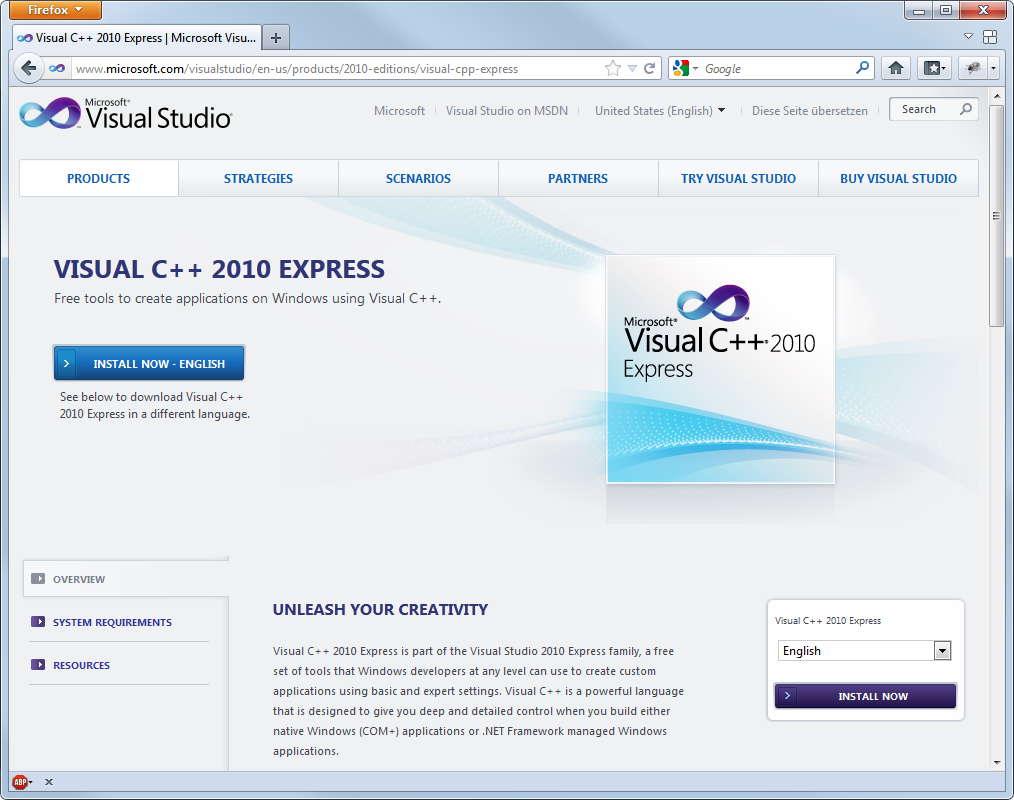
\includegraphics[scale=0.45]{figures/PNG/setup_vs_download1.png}
	\caption{Selecting Visual C++ 2010 Express for download.}
	\label{fig:setup_vs_download1}
\end{figure}

	\item Choose your language and click on \emph{Install}.
	
	\item If you are asked whether you want to install Visual Studio 2011 Professional instead,
		choose \emph{Visual C++ 2010 Express (English)} (compare Figure~\ref{fig:setup_vs_download2})\footnote{
		Alternatively, you can use the following direct link:\\
		\url{http://download.microsoft.com/download/1/D/9/1D9A6C0E-FC89-43EE-9658-B9F0E3A76983/vc_web.exe}}.

\begin{figure}[htbp]
	\centering
	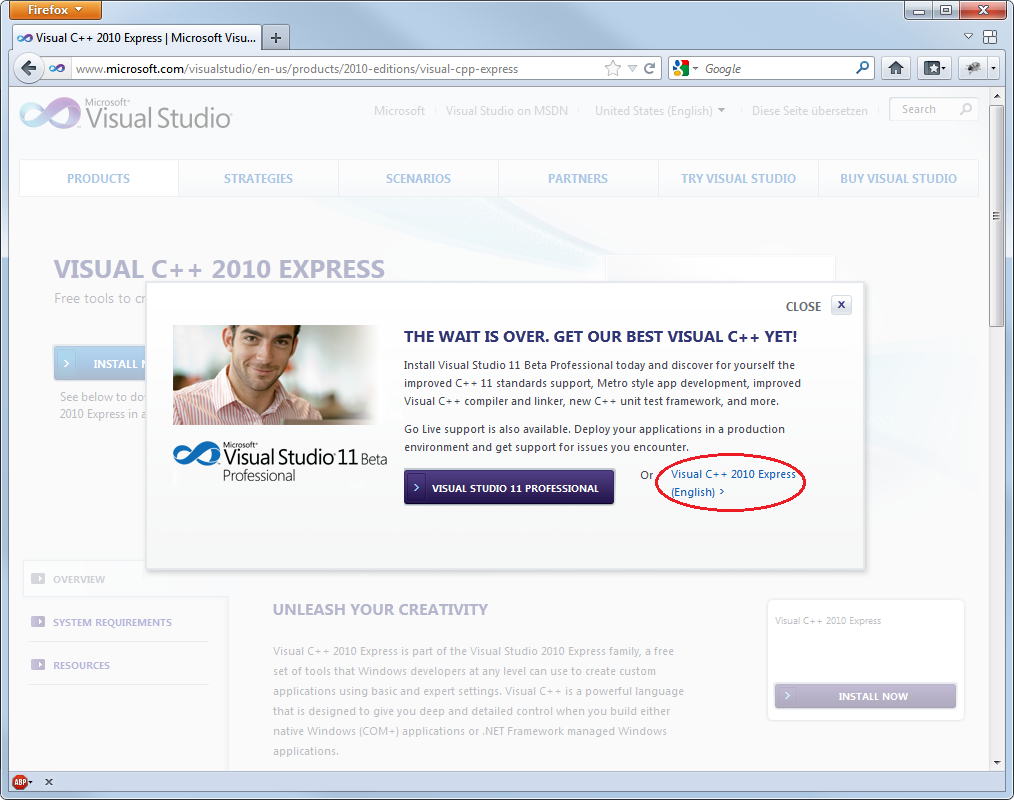
\includegraphics[scale=0.45]{figures/PNG/setup_vs_download2_edited.png}
	\caption{Downloading Visual C++ 2010 Express, highlighted in red the download link.}
	\label{fig:setup_vs_download2}
\end{figure}

	\item After downloading \texttt{vc\_web.exe}, launch it.
		Read the welcome screen and click \emph{Next} when ready. % (Figure~\ref{fig:setup_vs_welcome}).

%\begin{figure}[htbp]
%	\centering
%	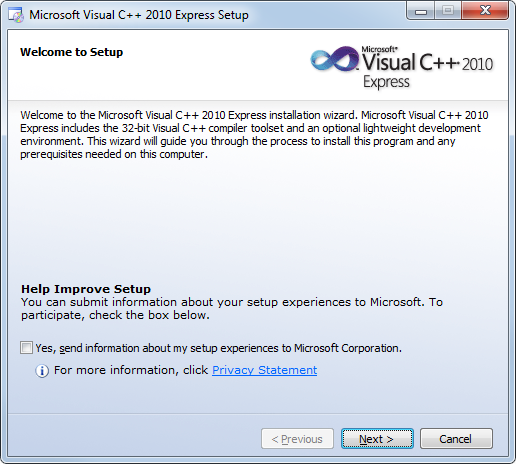
\includegraphics[scale=0.75]{figures/PNG/setup_vs_welcome.png}
%	\caption{Visual C++ 2010 Express setup welcome screen.}
%	\label{fig:setup_vs_welcome}
%\end{figure}

	\item Read the terms and conditions and choose the appropriate option. % (Figure~\ref{fig:setup_vs_terms}).

%\begin{figure}[htbp]
%	\centering
%	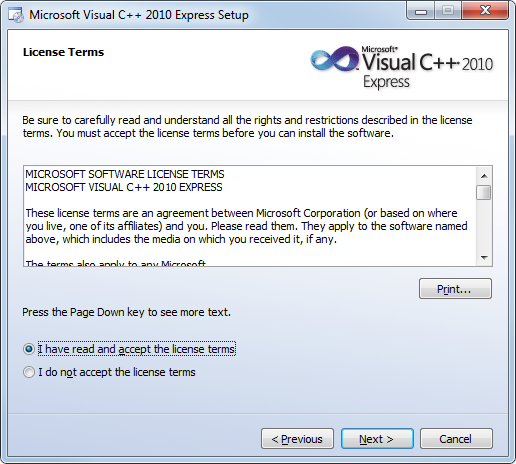
\includegraphics[scale=0.75]{figures/PNG/setup_vs_terms.png}
%	\caption{Visual C++ 2010 Express license terms.}
%	\label{fig:setup_vs_terms}
%\end{figure}

	\item On the \emph{Installation Options} page, you may deselect \emph{Silverlight} and \emph{SQL Server 2008}, they are not needed for \xme (Figure~\ref{fig:setup_vs_optional}).

\begin{figure}[htbp]
	\centering
	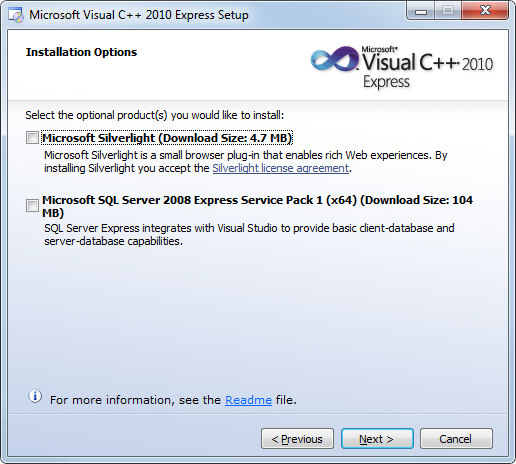
\includegraphics[scale=0.75]{figures/PNG/setup_vs_optional.png}
	\caption{Visual C++ 2010 Express installation options.}
	\label{fig:setup_vs_optional}
\end{figure}

	\item On the \emph{Destination Folder} page, select the installation directory.
		In some cases, you might not be able to choose a directory manually. % (compare Figure~\ref{fig:setup_vs_destination}).

%\begin{figure}[htbp]
%	\centering
%	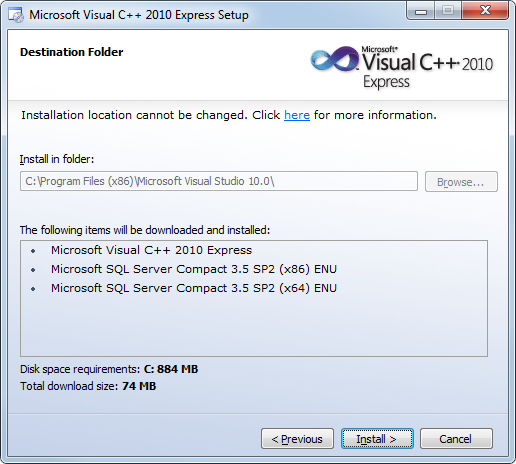
\includegraphics[scale=0.75]{figures/PNG/setup_vs_destination.png}
%	\caption{Visual C++ 2010 Express destination directory.}
%	\label{fig:setup_vs_destination}
%\end{figure}

	\item Wait for \emph{Visual C++} setup to finish downloading and installation. % (Figure~\ref{fig:setup_vs_install}).

%\begin{figure}[htbp]
%	\centering
%	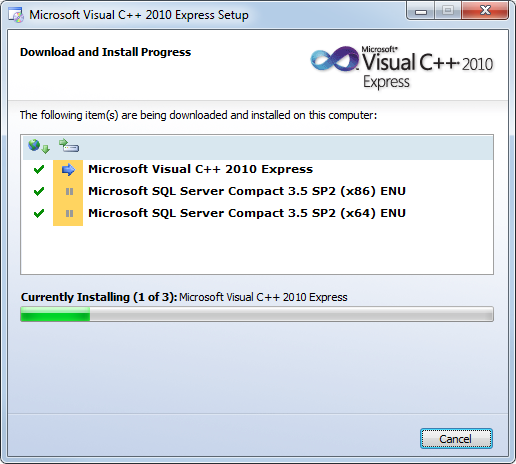
\includegraphics[scale=0.75]{figures/PNG/setup_vs_install.png}
%	\caption{Visual C++ 2010 Express download and install progress.}
%	\label{fig:setup_vs_install}
%\end{figure}

	\item After a few minutes, \emph{Visual C++} setup will report that the installation has finished. % (Figure~\ref{fig:setup_vs_success}).
		In some cases, a reboot may be required to use \emph{Visual C++}.

%\begin{figure}[htbp]
%	\centering
%	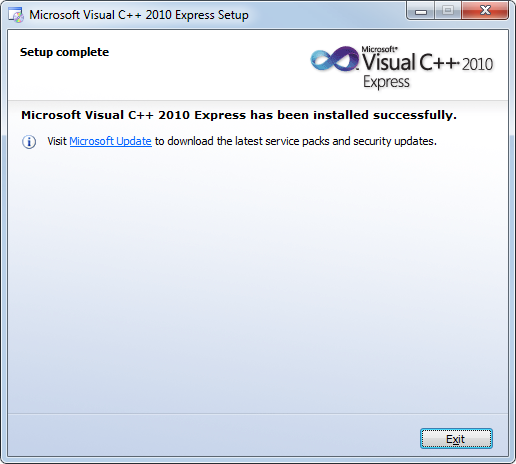
\includegraphics[scale=0.75]{figures/PNG/setup_vs_success.png}
%	\caption{Visual C++ 2010 Express setup complete.}
%	\label{fig:setup_vs_success}
%\end{figure}

\end{enumerate}
